% !TEX encoding = UTF-8
% !TEX TS-program = pdflatex
% !TEX root = ../tesi.tex

%**************************************************************
\chapter{Resoconto dello stage}
\label{cap:descrizione-stage}
%**************************************************************

\intro{In questo capitolo andrò a descrivere le principali tematiche ed attività che sono state affrontate durante il periodo di stage. Cercando di suddividere i vari processi in base alla loro utilità ed il loro scopo in ordine di percorrenza, in modo da spiegare le varie linee guida e metodologie attuate. }\\

%**************************************************************
\section{Introduzione al progetto}
Visto in scala più ampia, il progetto finale risulterà una rivisitazione di \textit{Bipod}, un applicativo di Siav, in ambito process mining, utilizzato come gestore di processi aziendali.
Tale software, dopo averlo provato con mano, risulta funzionante in ogni sua parte, anche se la sua struttura risulta poco estendibile. Per questo motivo mi è stato proposto di sviluppare una parte di software che si andrà poi ad integrare con il nuovo applicativo andando a rimpiazzare l'attuale esistente.
Nello specifico le principale richieste a cui ho fatto fronte sono state le seguenti:
\begin{itemize}
	\item Sviluppo di una libreria di process mining per filtraggio su log degli eventi.
	\item Sviluppo di un'nterfaccia fronted tenendo come punto di riferimento il vecchio applicativo.
	\item Scrittura di Stub per verificare il correntto comportamento dell'interfaccia di filtraggio.
\end{itemize}
La funzionalità che mi sono state proposte sono tra le più cruciali per quanto riguarda il prodotto finale, essendo le gestione dei filtri un'aspetto fondamentale nell'analisi dei processi. Per questo motivo è stato necessario investire una caspicua parte di tempo a disposizione per l'attività attività di formazione.
\section{Introduzione al \textit{Process mining}}
Il process mining è una tecnica di gestione dei processi attraverso il quale è possibile portare ad un miglioramento dei processi aziendali. I processi vengono analizzati attraversi particolari strutture chiamate log degli eventi. All'interno di tale struttura è presente una sequenza di eventi, che formano delle tracce. Una traccia può essere vista come un processo aziendale; un esempio utilizzato più volte è stato la produzione di un ingranaggio; individuando tutte le varie attività che avvengono partendo materiale grezzo fino ad arrivare al prodotto completo. Tramite l'analisi di tali processi è possibile studiare le varie procedure che intercorrono all'interno della realtà aziendale, cercando di osservare le varie dinamiche collegate ad ogni processo, per poi migliorarle ed ottimizzarle tramite un'analisi ben fatta tramite vari \textit{tool} presenti sul mercato. A questo merito \textit{Siav} ha deciso di fernire ai propri clienti un serivizio che sfruttasse questi principi.
\begin{figure}[!h] 
	\centering 
	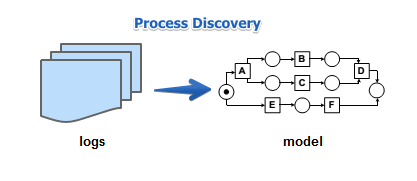
\includegraphics[width=0.8\columnwidth]{discovery} 
	\caption{Come viene rappresentato graficamente un log \url{http://mlwiki.org/index.php/Process_Mining}}
\end{figure}
\section{Pianificazione del progetto}
Durante la stesura del piano di lavoro sono state discusse con il tutor tutte le principali attività che avrei dovuto svolgere nell'arco dei due mesi preposti. Tali attività, anche se in forma generica, sono state inserite nel diagramma di Gantt presente al capitolo precedente (Figura 2.3).
Per tener entrare in maniera concreta all'interno dei processe aziendali, tramite il supporto del tutor e del team in cui sono stato inserito, ho cercato di apprendere nella miglior maniera possibile i principi cardine dell'\textit{Agile programming}. Non avendo mai avuto l'occasione prima d'ora di approcciarmi a tale metodologia è stato impegnativo, ma appagante entrare nei suoi meccanismi pratici e nelle sue dinamiche. Tuttavia sono riuscito, almeno in parte, a comprendere alcune importanti metodologie che sono state applicate durante tutto il periodo di stage. Le attività sono state tracciate tramite semplici note, condivise con l'interno team, in cui è descritta un breve cronologia di tutte le attività svolte giorno per giorno, indicando eventuali problematiche riscontrate e come sono state affrontate. La stessa motodologia è stata utilizzata per descrivere le tematiche trattate durante gli incontri di formazione e per descrivere le scelte fatte per far fronte alle diverse problematiche emerse.
Per poter verificare la corretta pianificazione era prassi organizzare \textit{Daily meeting} tra tutti i membri del team e gli stagisti presenti. In modo da potersi confrontare sullo stato di avanzamento del prodotto, discutendo di eventuale problematiche riscontrate e pianificando le attività per la giornata. In questo modo era possibile avere una panoramica generale sul prodotto ed un'opnione sul proprio operato da parte degli altri membri, capendo così la strada intrapresa fosse quella corretta.
\section{Studio preliminare}
In questa sezione sono descritte le principali attività svolte durante il periodo di formazione preliminare. Tale periodo è stato di fondamentale importanza per permettermi un buon grado di autonomia durante lo svolgimento di tutta l'attività di stage.
\subsection{\textit{Process mining}}
Prima di inoltrarsi all'interno del problema, è stato necessario un periodo di formazione che ha ricoperto la durata di due settimane, durante il quale ho appreso i principi cardine del \textit{process minig}, cercando di capire le sua dinamiche e la sua utilità all'interno di un contesto aziendale ben formato, per poter poi metterle in pratica all'interno del progetto. Tale periodo è stato caratterizzato dalla visioni di videolezioni online, per spiegare l'argomento in generale e da incontri programmati con il tutor in cui verificava il mio effettivo apprendimento. Inizialmente ho trovato difficoltà nell'apprendimento di tali nozioni, essendo stato per me un argomento completamente nuovo, ma dopo aver capito le sue meccaniche sono riuscito ad applicare in maniera completa i suoi principi durante tutte l'arco dello stage.
\subsection{Angular e \textit{typescript}}
In concomitanza con il periodo di formazine sopracitato sono stati svolti alcuni studi in merito al noto \textit{framewrok}, in modo da avere una buona base di partenza per poter procedere in autonomia allo sviluppo dell'interfaccia. Inizialmente, sotto consiglio del tutor ho guardato la documentazione presente all'interno del sito di Angular, in modo da poter avere una panoramica generale. Successivamente sono sono stato affiancato per un breve periodo da diverse figure all'interno dell'azienda, sviluppando alcune interfacce basilari che poi mi saranno state utili al fine del prodotto finale, in modo da rendere più metodica ed immediata l'assimilazione delle principali strutture presenti in Angular;
\section{Analisi dei requisiti}
Per poter tracciare i requisiti specifici necessari al compimento degli obiettivi, tramite consiglio del tutor mi sono servito dei principali \textit{tool di process mining} presenti sul mercato, assieme al software interno all'azienda \textit{Bipod}. In questo modo è stato possibile delineare una categorizzazione dei moduli di filtraggio richiesti, cercando di capire in che modo operassero nel concreto all'interno del log. Allo stesso modo sono stati tracciati ed analizzati i requisiti relativi all'interfaccia \textit{frontend}, confrontando le interfacce del loro applicativo con altri tool presenti in rete come \textit{ProM} e \textit{\gls{Disco}}. Per quanto riguarda lo \textit{stub} implementato è stato necessario uno studio preliminare dell'architettura finale, cercando di simularne il comportamento a seguito di richieste di filtraggi. 
\subsection{Libreria}
 Il \textit{tool} che mi ha permesso una maggior comprensione delle meccaniche di filtraggio, dandomi un buono spunto per l'implementazione della libreria è stato senz'altro \textit{ProM}; data la sua struttura modulare, a cui è possibile aggiungere esensioni di vario tipo, mi è stato possibile analizzarlo a fondo tramite lo studio del proprio repository. Mentre tramite gli altri \textit{tool} sono stato in grado di capire le dinamiche di filtraggio, tramite il repository di \textit{ProM} ho trovato alcuni esempi di implementazioni, anche se se mal documentati e poco comprensibili, cercando di aderire il più possibile allo standard. Nel caso della libreria, lo standard adottato è stato \textit{OpenXES}. Quest'ultimo rappresenta la struttura del log in formato .xes, una struttura molto simile ai file di tipo \textit{xml}. \textit{OpenXES} descrive il log degli eventi tramite una struttura dati chiamata XLog. A partire da questa struttura è possibile modellare i dati in arrivo a proprio piacimento gestendoli come vere e proprie lista di eventi. Tali eventi, rappresentati dalla classe XEvent, contengono un serie di attributi che vanno a caratterizzare l'evento e ne permettono il loro reperimento. I principali requisiti che sono emersi da questa analisi riguardano la categorizzazione delle tipologie di filtraggio, la loro implementazione ed il loro scopo. Sono state quindi delineate le seguenti tipologie:
\begin{itemize}
	\item Filtraggio basato su valori di TimeStamp
	\item Filtraggio basato sulle performance degli eventi.
	\item Filtraggio basato su eventi consecutivi
	\item Filtraggio basato sugli attributi
	\item Filtraggio basato sulle varianti
	\item Filtraggio basato su endpoint
\end{itemize}
\begin{figure}[!h] 
	\centering 
	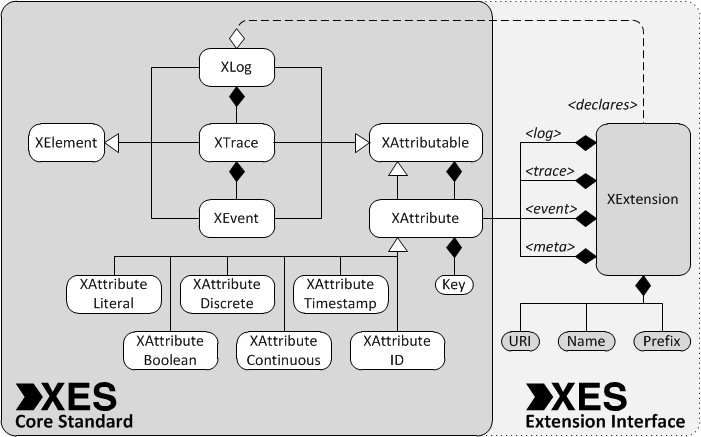
\includegraphics[width=0.9\columnwidth]{openxes} 
	\caption{Diagramma dei package dello standard openXes (\url{http://www.xes-standard.org/openxes/start})}
\end{figure}
Oltre alle funzionalità di filtraggio la libreria dovrebbe includere una serie di metodi legati al rilevamento di alcune caratteristiche del log in forma generica. In modo da poter determinare a priori alcune caratteristiche generali per poi agire di conseguenza.
Tali funzionalità di categorizzazione sono stata pensante per favorire all'interfaccia \textit{frontend} l'adattamento di fronte alle diverse tipologie di log che potevano venir esaminate dall'utente.
\subsection{\textit{Frontend}}
Per quanto rigurda i requisiti lato \textit{frontend} mi sono basato innanzitutto sullo studio dell'attuale \textit{tool} presente in azienda. Cercando di inquadrare in modo chiaro tutte le interfacce atte allo svolgimento di operazioni filtraggio. Dopo aver effettuato questa analisi, ho discusso a fondo in merito ad una specifica interfaccia, quella riguardante il filtraggio sulle performance. Il vecchio applicativo presentava un'interfaccia poco intuitiva in cui non era ben chiaro nè la sua utilità, ne le sue funzionalità. È stato quindi deciso di riscrivere l'interfaccia cercando di semplificare la visualizzazione attuale, redendo più piacevole ed intuitiva l'esperienza utente. Il risultato finale sarebbe quindi stata un'interfaccia solida ed intuitiva introducendo il supporto per le comunicazioni tramite \textit{\gls{Websocket}} e la gestione dei messaggi in arrivo dal server. Sono state quindi fissate le interfacce per ogni tipologia di filtraggio presente all'interno della libreria.

\subsection{\textit{Stub}}
Dopo la fase di negoziazione dei requisiti con il tutor aziendale, è stato deciso in comune accordo con il tutor che la parte riguardante l'architettura del \textit{Backend} venisse accantonata dato il tempo limitato a mia dispoizione e la sua rilevante complessità, per far spazio ad uno \textit{Stub} che andasse a simulare il comportamento dell'architetture finale a fronte di una richiesta di filtraggio. Tale \textit{Stub} avrebbe dovuto comunicare con il \textit{Client} tramite un canale \textit{Websocket}, andando a gestire tutte le tipologie di messaggi ritornati dal server.
\begin{figure}[!h] 
	\centering 
	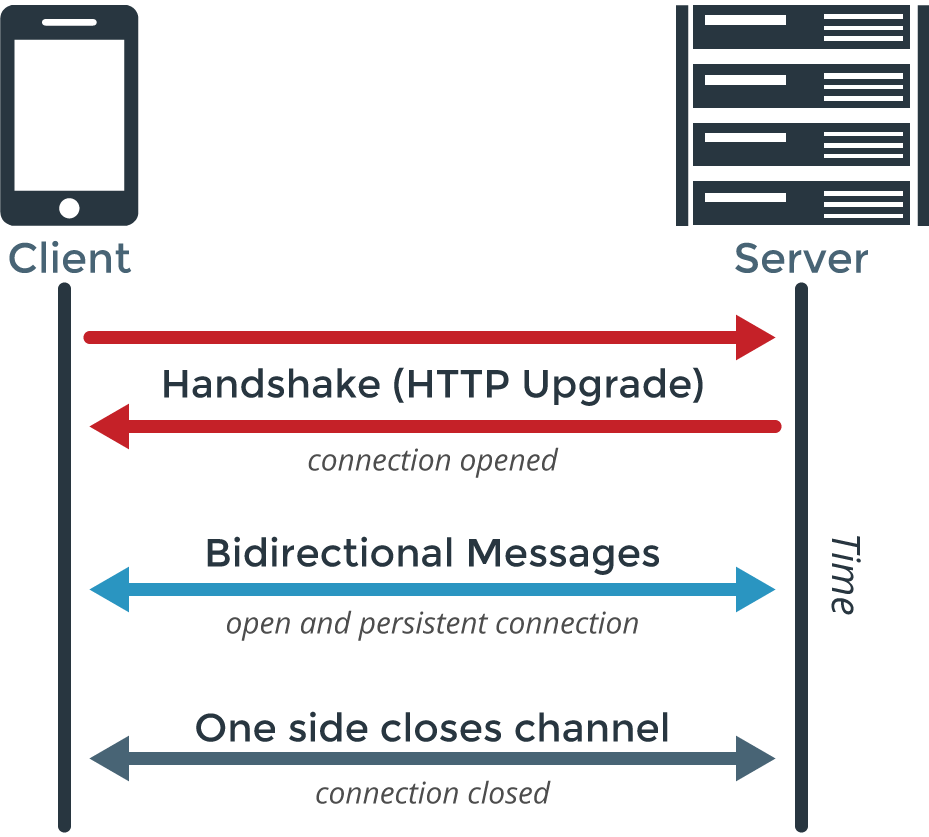
\includegraphics[width=0.6\columnwidth]{websocket} 
	\caption{Ciclo di vita di una connessione tramite websocket \url{https://radu-matei.com/blog/aspnet-core-websockets-middleware/}}
\end{figure}
\newpage
\section{Progettazione}
\subsection{Libreria}
Dopo aver delineato i principali requisiti da dover soddisfare sono passato alla fase di progettazione, cercando di strutturare la libreria in modo semplice, ma allo stesso tempo efficace, andando a documentare ogni singola funzionalità tramite \textit{\gls{Javadoc}}, in modo da rendere mantenibile l'intera libreria e soprattutto di facile comprensione ai futuri utilizzatori. È stato deciso di dividerla in più classi, ognuna di esse riguardante una tipologia di filtraggio in modo da rendere la letture della libreria più semplice ed immediata. Tutti i metodi presenti all'interno della libreria operavano su tipi di dato in formato standard derivati da \textit{OpenXES}, questo è stato un requisito fortemente richiesto dal tutor interno. Oltre alle operazioni di filtraggio sono state inclusi altri metodi per poter effettuare degli studi preliminare sul log preso in esame, andando a catalogarlo sotto determinati aspetti che, al fine di tutto l'applicativo, risultano di fondamentale importanza.
\subsection{\textit{Frontend}}
Per poter eseguire una fase di Progettazione trasparente rispetto ai requisiti analizzati mi sono avvalso di alcuni \textit{mockup} tramite il quale, sotto la supervisione del tutor, sono andato a tracciare tutte le interfacce di filtraggio, andando a rispettare tutti i requisiti preposti. Tali modelli sono stati ideati allo stesso modo con cui è stata progettata la libreria; utilizzando un \textit{layout} a schede, in cui, per ogni scheda è presente una tipologia di filtraggio. Come per la fase di analisi dei requisiti anche in questo caso il filtraggio sulle performance ha richiesto una particolare attenzione: nel vecchio applicativo tale interfaccia era mal strutturata e non era ben chiaro all'utente che tipo di filtraggio stesse utilizzando. Ciò era dovuto ad un aspetto che prima d'ora non è stato preso in considerazione: il \textit{lifecycle} delle attività. Questo aspetto ha portato ad un lunga discussione con il tutor ed i membri del team in merito alle scelte da adottare. Ne è emerso che sarebbe stato necessario una differente interfaccia utente in base alla tipologie di lifecycle presente all'interno del log. Tali metodi sono stati opportunamente implementati all'interno della libreria.\\
Per quanto rigurarda l'interazione con i servizi \textit{backend} è stato necessario avvalersi di \textit{RxJS}; una libreria sviluppata per \textit{javascript} che presenta tutte le principali funzionalità per la gestione dei messaggi tramite canali \textit{websocket}. Questa libreria è in grando di riperire i messaggi in arrivo tramite un gestore di \textit{callback} che differenzia i vari messaggi e fa reagire l'interfaccia in modo diverso a seconda della tipologia in arrivo.

\subsection{\textit{Stub}}
Prima di poter passare alle realizzazione dello Stub è stato necessario dare una particolare attenzione all'architettura finale del backend. Purtroppo, date le strette tempistiche da rispettare e le varie criticità riscontrate durante le fasi precedenti è stato possibile comprenderla solamente a livello teorico. Tale architettura si basava quindi su un sistema a microservizi. All'interno di essa erano presente degli \textit{worker} che reagivano a determinate richieste lato \textit{client}. Nel momento in cui veniva presa in carico l'operazione il \textit{worker} ritornava messaggi di progresso, che andavano quindi ag aggiornare l'interfaccia. Al momento della terminazione, il servizio inviava il relativo messaggio, che andava a notificare l'utente sull'effettivo completamento dell'operazione di filtraggio. Dopo aver appreso tali dinamiche ho potuto definire uno Stub che rispettasse le caratteristiche descritte.
\begin{figure}[!h] 
	\centering 
	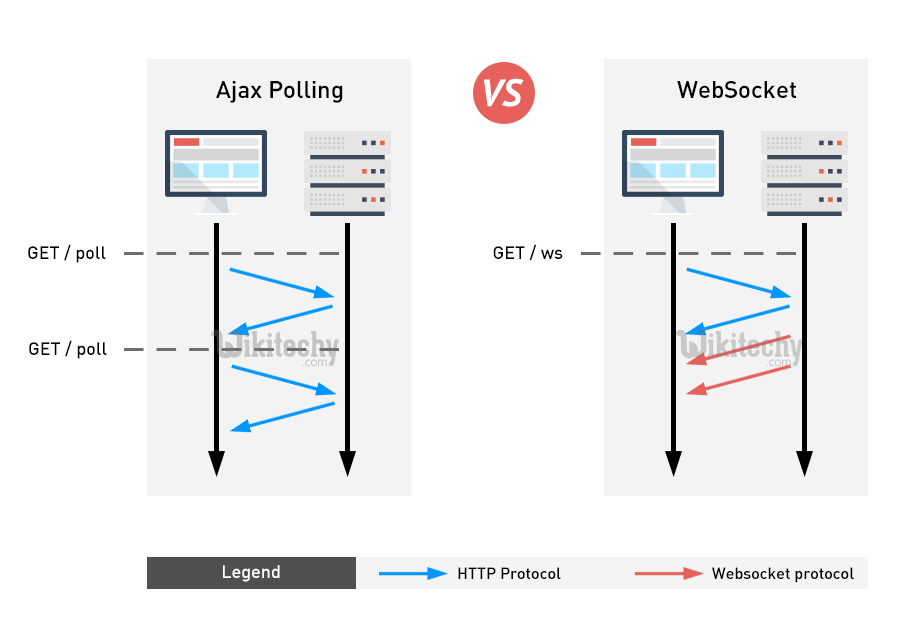
\includegraphics[width=0.9\columnwidth]{websocket-vs-ajax} 
	\caption{Differenza tra una chiamata websocket ed una http \url{https://www.wikitechy.com/tutorials/socket/differences-between-websockets-and-ajax}}
\end{figure}
\newpage
\section{Codifica}
libreria (problemi performance), typescript e angular(problemi coon alcuni componenti)
\section{Copertura}
unit test per tutte le funzionali della libreria confrontando con quanto mi usciva da disco.
\section{Verifica}
controllo da parte del tutor
\section{Validazione}
approvazione finale da parte del tutor